% !TEX root = ../document.tex
% !TeX spellcheck = pt_BR

% ----------------------------------------------------------
\chapter[Noções de processamento de sinais]{Noções de processamento de sinais}
\thispagestyle{empty}
\label{chap:chapter3}
% ----------------------------------------------------------

Um pequeno ferramental matemático necessário para entender o tratamento de sinais digitais será apresentado neste capítulo. Num primeiro momento serão vistos conceitos como espaços, bases ortonormais e aproximação de vetores. Depois, a transformada de Fourier de tempo discreto e sua generalização, a transformada z, serão apresentadas. Em seguida, será feita uma breve discussão sobre a questão do projeto de filtros digitais. Por fim, serão discutidos os polinômios de Hermite e a expansão em funções de Hermite. Isto visa permitir um melhor entendimento dos próximos capítulos. Contudo, o leitor, se desejar, pode se referir apenas ao resumo no final do capítulo e prosseguir com a leitura do trabalho.


\section{Representação de sinais discretos}
\label{sec:discretesig}
Um sinal discreto $x[n]$ é uma sequência de valores em $\mathbb{R}$ ou $\mathbb{C}$, alocados em instantes de tempo discreto $n$. Normalmente, esta sequência representa as amplitudes geradas por um instrumento de medição sobre um processo físico qualquer, depois de amostradas e quantizadas por um conversor analógico-digital (A/D). Em particular, estamos interessados em processos reais (sem parte imaginária) e estocásticos, isto é, que não possuem comportamento previsível mas possuem propriedades estatísticas que os descrevem. Nas próximas subseções, verá-se como um sinal deste tipo pode ser decomposto em funções mais simples e conhecidas e também como se pode utilizar um conjunto finito e reduzido destas funções para aproximá-lo. Para um tratamento mais completo do assunto, sugere-se referir ao capítulo 2 do livro \cite{Vetterli1995}.

\subsection*{Espaços, bases e ortogonalidade}
Na álgebra linear, costumamos tratar espaços vetoriais de dimensões finitas, como $\mathbb{R}^n$ ou $\mathbb{C}^n$. Neste contexto, dado um conjunto de vetores ${v_k}$, desejamos responder a perguntas como:
\begin{itemize}
    \item o espaço em questão é \emph{gerado} (\emph{spanned}) pelo conjunto ${v_k}$? Em outras palavras, qualquer vetor no espaço pode ser representado por uma combinação linear de vetores de ${v_k}$?
    \item os vetores são linearmente independentes? Isto é, a afirmação de que um vetor em ${v_k}$ pode ser escrito como combinação linear dos demais é falsa?
    \item como é possível encontrar bases e, em particular, bases ortonormais, que geram o espaço?
    \item por fim, dado um subespaço e um vetor qualquer, como podemos encontrar uma aproximação para esse vetor no subespaço?
\end{itemize}

Para respondê-las, utilizamos as noções de \textbf{norma} (ou tamanho) e \textbf{ortogonalidade} de vetores. Dados dois vetores $x$ e $y$ no espaço $\mathbb{R}^n$, temos:
\begin{itemize}
    \item a norma quadrada: $\|x\| = \sqrt{\sum_{i=1}^{n} x^2_i}$
    \item o produto escalar: $\langle x,y \rangle = \sum_{i=1}^{n} x_iy_i$
    \item a propriedade de ortogonalidade: $\langle x,y \rangle = 0$
\end{itemize}

Quando se trabalha com espaços infinitamente dimensionais, fala-se de uma extensão da álgebra linear, que são os espaços de Hilbert. Um espaço de Hilbert é um espaço vetorial de dimensões possivelmente infinitas, equipado com um operador \textbf{produto interno}. Podemos escrever o produto interno $\langle\cdot,\cdot\rangle$ para o caso de sequências reais como:
\begin{equation}
    \langle x,y \rangle = \sum_{n=-\infty}^{\infty} x[n]y[n]
    \label{equ:innerprod}
\end{equation}

Este operador é linear, pois satisfaz as propriedades de aditividade $\langle x+y,z \rangle = \langle x,z \rangle + \langle y,z \rangle$ e homogeneidade $\langle x,\alpha y \rangle = \langle \alpha x,y \rangle = \alpha\langle x,y \rangle$, para $\alpha \in \mathbb{R}$. Também satisfaz $\langle x,x \rangle \geq 0$, e $\langle x,x \rangle = 0$ se $x=0$. Podemos usar o produto interno para definir normas e ortogonalidade. A norma de um vetor é escrita como $\|x\| = \sqrt{\langle x,x \rangle}$ e a distância entre dois vetores $x$ e $y$, como a norma de sua diferença $\|x-y\|$. Podemos ainda dizer que $x$ e $y$ são ortogonais, $x\perp y$, se $\langle x,y \rangle = 0$.

Precisamos também definir o conceito de base. Um subconjunto $S=\{x_1,\ldots,x_n\}$ de um espaço vetorial $E$ forma uma \textbf{base} para $E$ se o espaço é gerado por $S$ e se $x_i,\ldots,x_n$ são linearmente independentes. No caso de um espaço de dimensões infinitas, $S$ deve conter infinitos vetores linearmente independentes. Por exemplo, o conjunto $\{\delta[n-k]\}_{k\in\mathbb{Z}}$, em que $\delta[n]$ é a função impulso discreto unitário, forma uma base para o espaço de sequências infinitas, pois possui infinitos vetores linearmente independentes que geram este espaço.

Um caso especial é quando os vetores da base são ortogonais entre si e possuem norma unitária. Diz-se então que a base é ortonormal. O procedimento para se encontrar uma base ortonormal a partir de um conjunto de vetores linearmente independentes (que geram o espaço de interesse) é chamado de ortogonalização de Gram-Schmidt. Essencialmente, tem-se
\begin{equation}
    y_k = \frac{x_k-v_k}{\|x_k-v_k\|},
\end{equation}
onde $v_1 = 0$, e
\begin{equation}
    v_k = \sum_{i=1}^{k-1} \langle y_i,x_k\rangle y_i,\quad k=2,3,\ldots
\end{equation}
são as projeções sucessivas de um vetor do conjunto no subespaço gerado pelos vetores previamente ortogonalizados. Como será visto a seguir, esta expressão dá a melhor aproximação de um vetor no subespaço.


\subsection*{Aproximação por mínimos quadrados}

Dado um vetor $y$ num espaço $E$, deseja-se encontrar uma aproximação para este vetor que esteja num subespaço $S \subset E$. Assumindo que $S$ possua uma base ortonormal $\{x_1,x_2,\ldots\}$, a projeção ortogonal de $y \in E$ em $S$ é dada por
\begin{equation}
    \hat{y} = \sum_{i} \langle x_i,y\rangle x_i.
\end{equation}
A diferença $d=y-\hat{y}$ está no complemento ortogonal de $S$ e, em particular, $d$ é ortogonal a $\hat{y}$. Esta relação pode ser facilmente visualizada no espaço Euclideano tridimensional, conforme mostra a figura \ref{fig:three-dim}. Pela mesma figura, é possível ver que
\begin{equation}
    \|y\|^2 = \|\hat{y}\|^2+\|d\|^2.
\end{equation}
A aproximação é ótima no sentido de mínimos quadrados, isto é, o valor $min\|y-x\|$ para $x$ em $S$ e $y=\sum_{i} \alpha_ix_i$ é obtido com
\begin{equation}
    \alpha_i = \langle x_i,y\rangle.
\end{equation}
Os $\alpha_i$ são chamados coeficientes da expansão de $y$ em termos de $x_i$.

\begin{figure}[ht!]
    \centering
    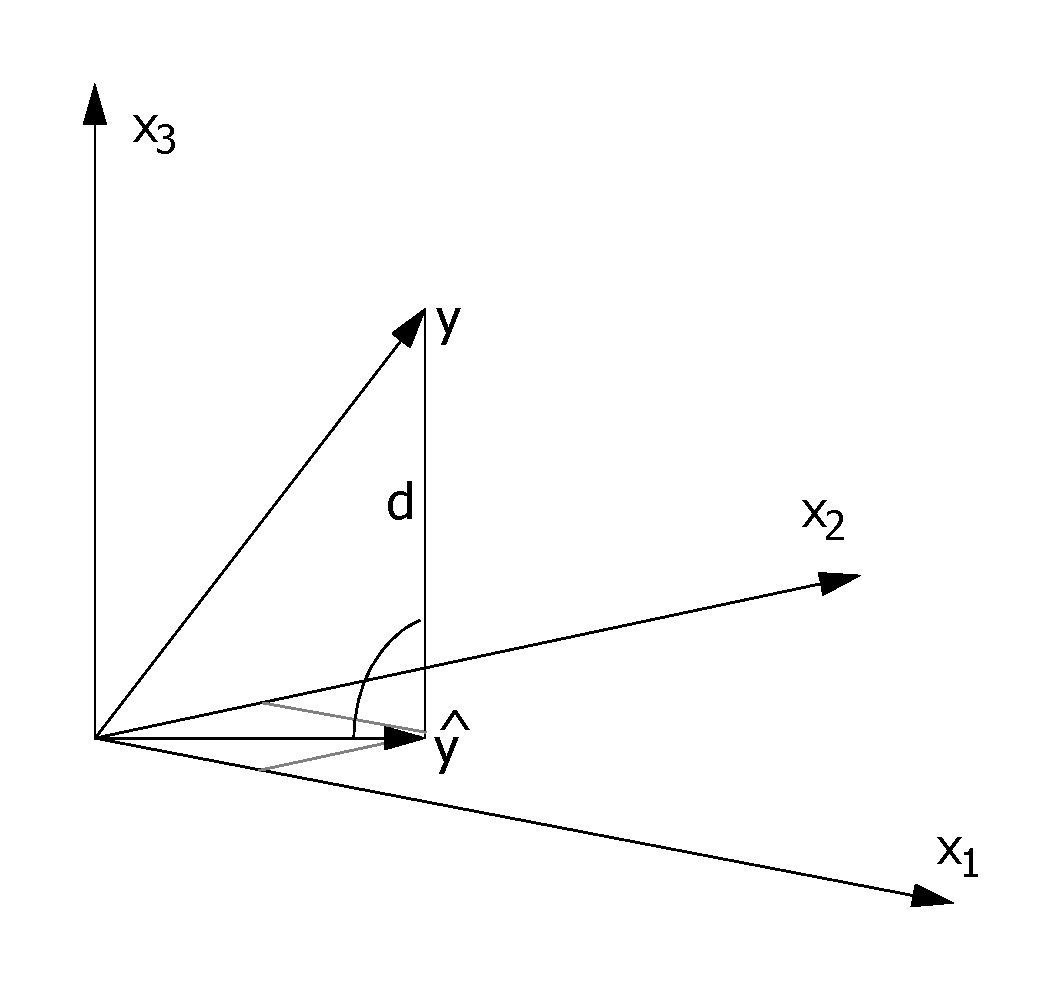
\includegraphics[width=200pt]{figures/chap3-three-dim.pdf}
    \caption[Projeção no espaço tridimensional]{Projeção no espaço tridimensional. Extraída de \cite{Vetterli1995}.}
    \label{fig:three-dim}
\end{figure}

A seguir será introduzida uma metodologia de representação de sinais discretos que usa como base a sequência de polinômios de Hermite. Esta técnica será utilizada em dois dos métodos de detecção de isquemia, conforme será visto nos capítulos \ref{chap:chapter5} e \ref{chap:chapter6}.

\subsection*{Polinômios de Hermite}
Os polinômios de Hermite podem ser obtidos pela seguinte relação de recorrência:
\begin{equation}
     \begin{array}{l}
         H_0(x) = 1\\
         H_1(x) = 2x\\
         H_{n+1}(x) = 2xH_n(x) - 2nH_{n-1}(x), \quad n \geq 1
     \end{array}.
\end{equation}
Ou podem ser expressos de forma explícita (não recursiva) por
\begin{equation}
     H_n(x) = n! \sum_{m=0}^{\lfloor \frac{n}{2} \rfloor} \frac{\left(-1\right)^m}{m!\left(n-2m\right)!}\left(2x\right)^{n-2m}.
\end{equation}
Os polinômios de Hermite são ortogonais entre si com respeito à função $e^{-x^2}$. Tomando o produto interno por esta métrica, tem-se:
\begin{equation}
     \int_{-\infty}^{\infty} H_m(x)H_n(x)e^{-x^2}dx = 0, \quad m\neq n
\end{equation}
Note aqui o uso da integral em vez do somatório (ver equação \ref{equ:innerprod}), por conta da variável $x$ ser contínua. Os primeiros seis polinômios de Hermite são descritos abaixo e têm seu gráfico mostrado na figura \ref{fig:hermpoly}.
\begin{equation}
     \begin{array}{l}
         H_0(x) = 1\\
         H_1(x) = 2x\\
         H_2(x) = 4x^2 - 2\\
         H_3(x) = 8x^3 - 12x\\
         H_4(x) = 16x^4 - 48x^2 + 12\\
         H_5(x) = 32x^5 - 160x^3 + 120x
     \end{array}
\end{equation}

\begin{figure}[ht!]
    \centering
    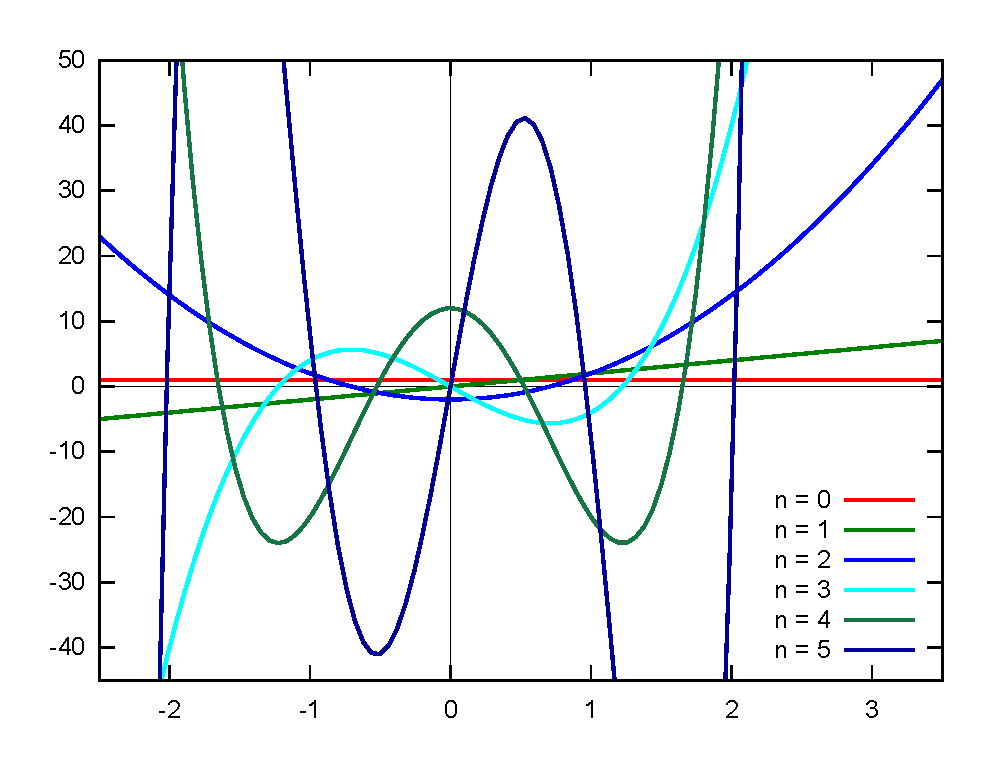
\includegraphics[width=300pt]{figures/chap3-herm-polynomials.pdf}
    \caption[Gráfico dos primeiros seis polinômios de Hermite]{Gráfico dos primeiros seis polinômios de Hermite. Extraído de \cite{Damato2009}.}
    \label{fig:hermpoly}
\end{figure}


\subsection*{Expansão em funções de Hermite}
As funções de Hermite são definidas em termos dos polinômios de Hermite, de acordo com a equação \ref{equ:hermfunc} abaixo. A figura \ref{fig:hermfunc} mostra o gráfico das primeiras seis funções.
\begin{equation}
    \psi_n(x) = \left(\frac{e^{-x^2}}{n!2^n\sqrt{\pi}}\right)^\frac{1}{2} H_n\left(x\right)
    \label{equ:hermfunc}
\end{equation}
De acordo com a teoria descrita em \cite{Abramowitz1974}, seguindo também o raciocínio introduzido para os polinômios de Hermite, essas funções são ortogonais entre si. Tomando o produto interno, tem-se:
\begin{equation}
     \int_{-\infty}^{\infty} \psi_m(x)\psi_n(x)dx = 0, \quad m\neq n.
\end{equation}
As funções de Hermite formam uma base ortonormal para o espaço de funções integráveis ao quadrado, $L^2(\mathbb{R})$. Portanto, têm aplicação direta na expansão de sinais desse tipo.

\begin{figure}[ht!]
    \centering
    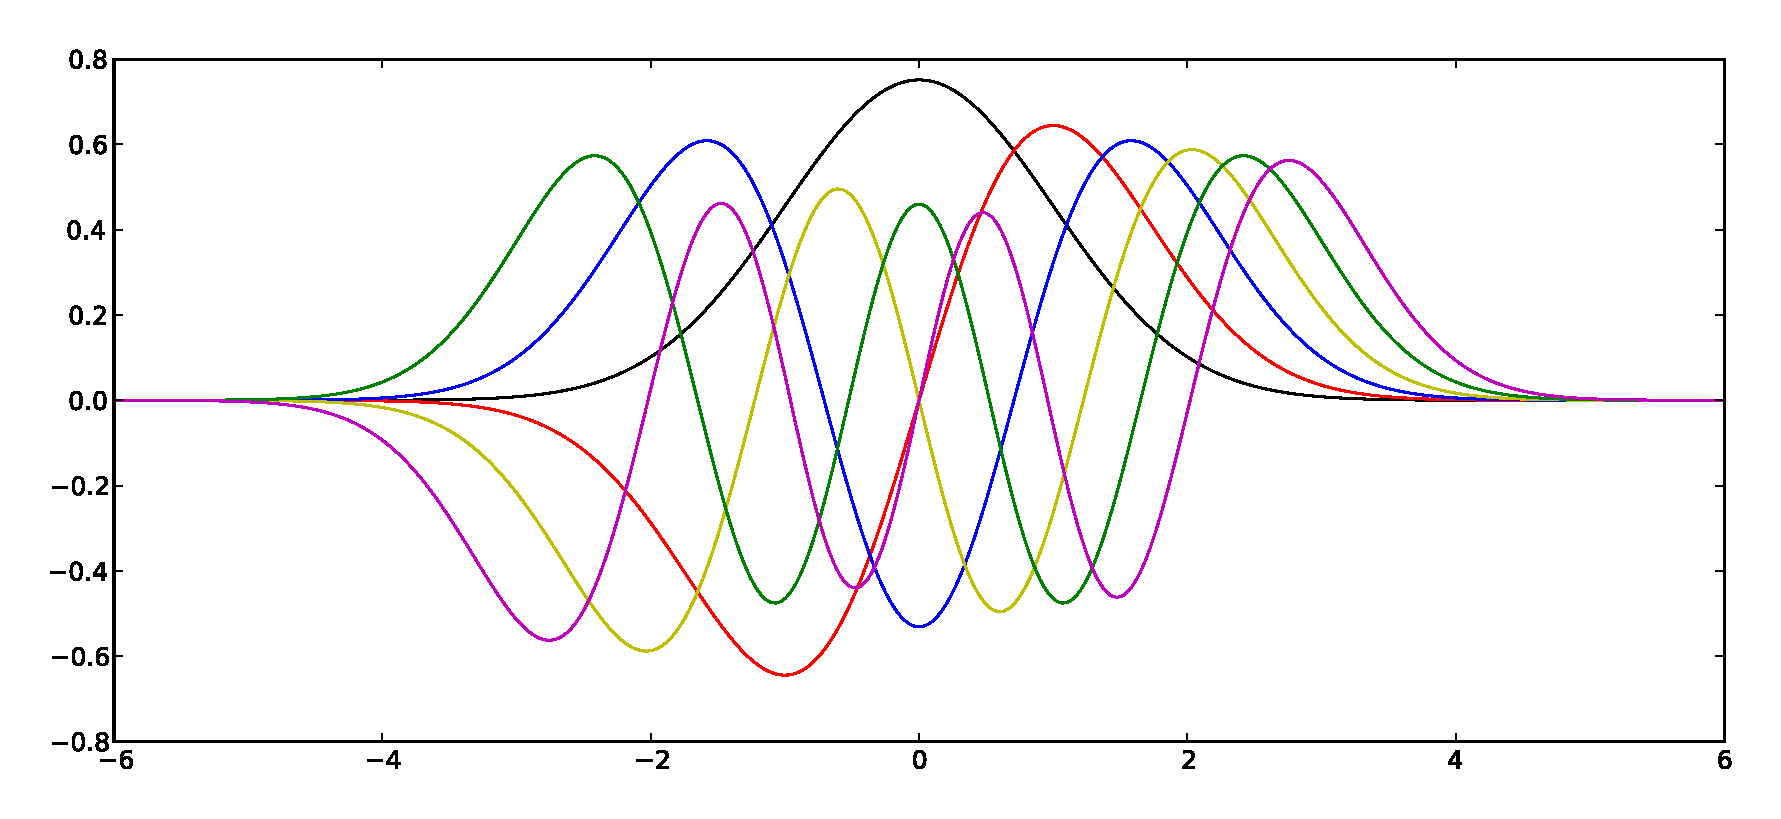
\includegraphics[width=400pt]{figures/chap3-herm-functions.pdf}
    \caption[Gráfico das primeiras seis funções de Hermite]{Gráfico das primeiras seis funções de Hermite. Extraído de \cite{Dems2009}.}
    \label{fig:hermfunc}
\end{figure}

No caso discreto, precisamos adotar uma abordagem um tanto diferente de cálculo dessas funções, que advém do fato delas serem autofunções da transformada de Fourier. Segundo a técnica descrita em \cite{Mugler2002}, as funções discretas de Hermite são autovetores de uma matriz tridiagonal e simétrica $T_b$. Esta matriz é completamente especificada por sua diagonal principal e diagonal secundária, cujos elementos são dados por
\begin{equation}
    d_{0,i} = -2\cos(N\pi\tau)\sin(i\pi\tau)\sin((N-i-1)\pi\tau), \quad 0\leq i\leq N-1
    \label{equ:maindiag}
\end{equation}
e
\begin{equation}
    d_{1,k} = \sin(k\pi\tau)\sin((N-k)\pi\tau), \quad 1\leq k\leq N-1,
    \label{equ:offdiag}
\end{equation}
onde $\tau = \frac{1}{Nb^2}$, $b$ é um parâmetro de dilatação e $N$ é o tamanho do sinal. O efeito do parâmetro $b$ é um alargamento das funções de Hermite no eixo temporal, à medida que $b$ aumenta.

Os autores advogam que o maior autovalor da matriz $T_b$ (num ordenamento do maior para o menor), corresponde à primeira função discreta de Hermite; o segundo maior autovalor, à segunda função de Hermite e assim por diante. Logo, o algoritmo de cálculo das funções discretas de Hermite consiste em construir a matriz $T_b$ conforme as equações \ref{equ:maindiag} e \ref{equ:offdiag}, extrair-lhe os autovetores e autovalores e, finalmente, enumerar os autovetores de acordo com seus respectivos autovalores em ordem decrescente. Uma vez normalizados (norma unitária), estes vetores formam uma base ortonormal para o espaço de sequências somáveis ao quadrado, $L^2(\mathbb{Z})$.

A expansão de $x[n]$, com $0\leq n\leq N-1$, por funções de Hermite se dá pelo produto interno de $x$ com cada um dos vetores previamente calculados. Podemos ainda construir uma matriz $U$ tendo esses vetores como linhas. Então a expansão se resume a um produto matricial $Ux$. Note que $x$, assim como $U$, possui dimensões finitas e, portanto, esta operação é na verdade uma aproximação. Em outras palavras, ela é a projeção de $x$ no subespaço gerado pelas linhas de $U$. A figura \ref{fig:hermexp} ilustra em linha pontilhada a aproximação de um sinal discreto (representado, por conveniência, usando linha contínua) usando as 50 primeiras funções discretas de Hermite.

\begin{figure}[ht!]
    \centering
    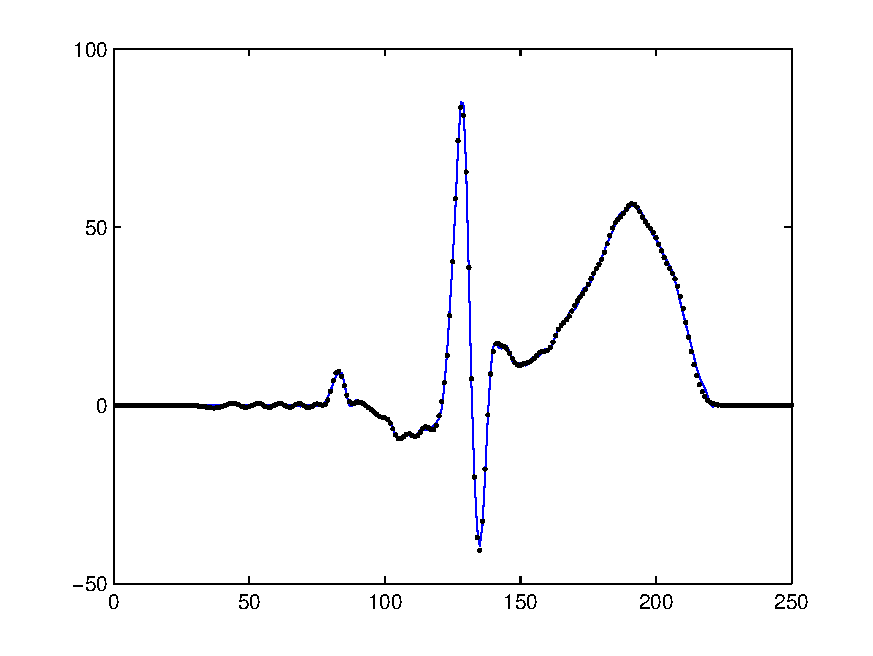
\includegraphics[width=400pt]{figures/chap3-herm-expansion.pdf}
    \caption[Gráfico da expansão usando 50 funções de Hermite]{Gráfico da expansão usando 50 funções de Hermite. Produzido no MATLAB.}
    \label{fig:hermexp}
\end{figure}


\section{Transformadas de tempo discreto}

A transformada de Fourier é uma ferramenta versátil de análise de sinais, pois evidencia componentes de frequência existentes num sinal e permite manipulá-lo por meio dessas componentes. Nesta subseção serão introduzidas a transformada de Fourier de tempo discreto e sua generalização, a transformada z. Ambas constituem o fundamento para a análise de sinais discretos no domínio frequencial, inclusive no que tange ao projeto de filtros digitais, assunto da seção consecutiva. A base para a discussão que segue, tanto nesta seção como na \ref{sec:filterdesign}, vem do livro \cite{Oppenheim2009}.

\subsection*{Transformada de Fourier de tempo discreto}
A transformada de Fourier de tempo discreto (DTFT) é definida como
\begin{equation}
     X(e^{j\omega}) = \sum_{n=-\infty}^{\infty} x[n]e^{-j\omega n}.
     \label{equ:dtft}
\end{equation}
Sua inversa, ou seja, a operação que fornece $x[n]$ a partir de $X(e^{j\omega})$ é
\begin{equation}
     x[n] = \frac{1}{2\pi}\int\limits_{(2\pi)} X(e^{j\omega})e^{j\omega n}.
\end{equation}

A equação \ref{equ:dtft} pode ser entendida como a relação que dá os coeficientes da expansão de $x[n]$ em funções exponenciais complexas, sendo estas as componentes de uma base para o espaço de sequências infinitas (e somáveis ao quadrado). A variável $\omega$ tem unidade em radianos.

\subsection*{Transformada z}

A transformada z é definida como
\begin{equation}
     X(z) = \sum_{n=-\infty}^{\infty} x[n]z^{-n},
\end{equation}
onde $z$ é, em geral, um número complexo: $z=Ae^{j\phi}$.

Por vezes, estamos interessados na representação de um sistema linear e invariante no tempo (LIT) através da transformada z, em cujo caso expressamos a equação de diferenças do sistema,
\begin{equation}
     \sum_{k=0}^{N} a_ky[n] = \sum_{k=0}^{M} b_kx[n],
\end{equation}
na forma (usando as propriedades de linearidade e deslocamento no tempo da transformada):
\begin{equation}
     Y(z)\sum_{k=0}^{N} a_kz^{-k} = X(z)\sum_{k=0}^{M} b_kz^{-k}.
\end{equation}
Podemos ainda escrever a função de transferência (ou resposta em frequência) do sistema como
\begin{equation}
     H(z) = \frac{Y(z)}{X(z)} = \frac{\sum_{k=0}^{M} b_kz^{-k}}{\sum_{k=0}^{N} a_kz^{-k}}.
     \label{equ:zresp}
\end{equation}

A equação \ref{equ:zresp} também pode ser rearranjada para evidenciar as raízes do polinômio numerador e do polinômio denominador, chamadas de zeros e pólos, respectivamente. Os zeros e pólos indicam os pontos onde a resposta em frequência do sistema cai a zero ou tende ao infinito. Eles são mais facilmente visualizados no \textbf{plano z}, conforme mostra a figura \ref{fig:zplane}. O plano z é uma ferramenta indispensável na análise de estabilidade e causalidade de sistemas discretos, bem como no projeto de filtros digitais, conforme será discutido na próxima seção.

\begin{figure}[ht!]
    \centering
    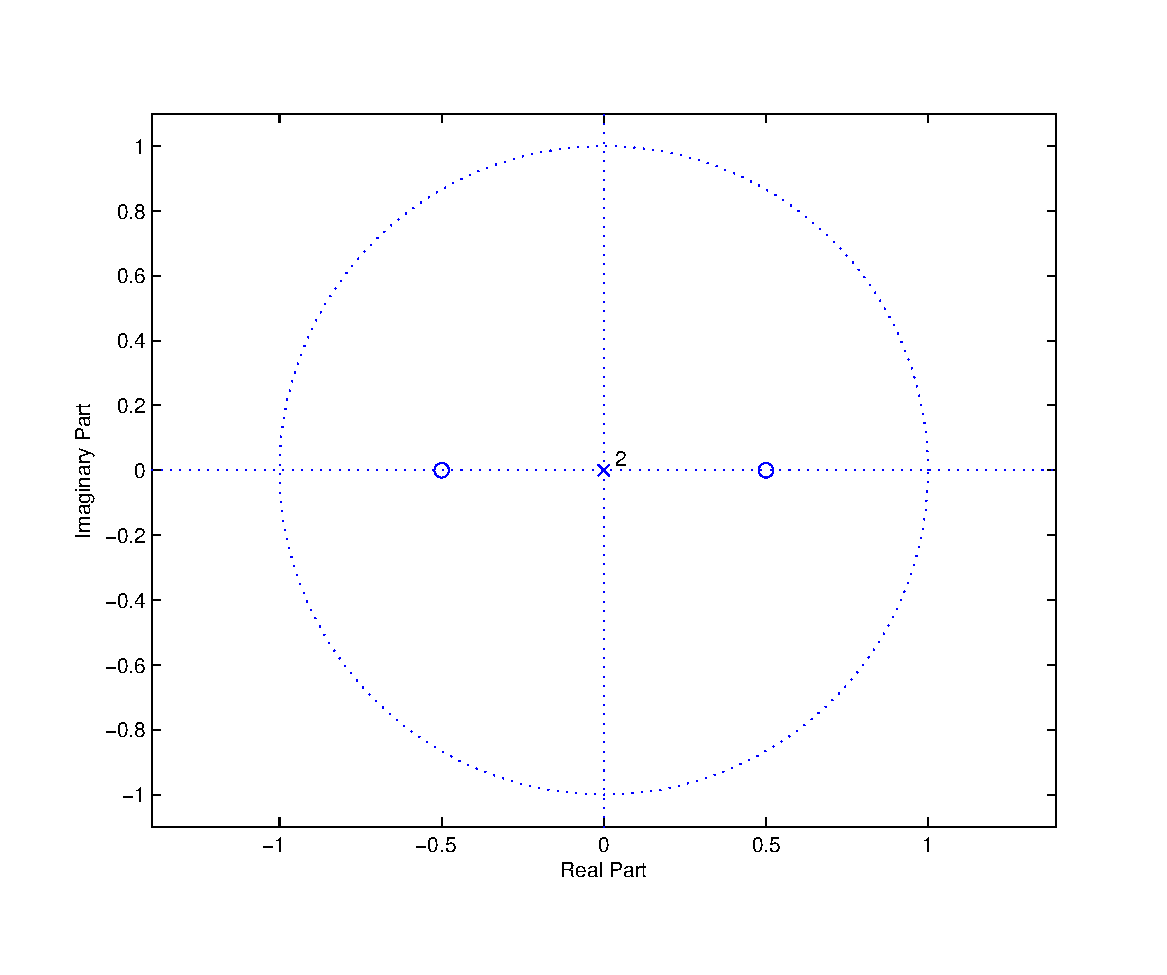
\includegraphics[width=300pt]{figures/chap3-z-plane.pdf}
    \caption[Plano z]{Plano z. Pólos duplos em $z=0$ e zeros em $z=\pm 0.5$.}
    \label{fig:zplane}
\end{figure}


\section{Projeto de filtros digitais}
\label{sec:filterdesign}
Filtros digitais têm uma grande variedade de aplicações, tanto na área biomédica quanto em qualquer outra que requeira processamento de sinais digitais. Neste trabalho, deseja-se manipular um sinal de ECG com vistas à detecção de batimentos cardíacos e também filtrá-lo para remover ruído e interferência da rede elétrica (50 ou 60 Hz). Esta seção apresenta alguns conceitos sobre o projeto de filtros digitais que auxiliarão o leitor no entendimento dos próximos capítulos, sobretudo no que tange à etapa de pré-processamento dos métodos de detecção de isquemia.

\subsection*{Tipos de filtros}
Há duas categorias básicas de filtros: o de resposta impulsiva finita (FIR) e o de resposta impulsiva infinita (IIR). O primeiro diz respeito àqueles filtros cuja resposta depende apenas da entrada em diferentes instantes de tempo. Em outras palavras, a equação de diferenças que descreve o comportamento do filtro não possui termos em $y[n-k], k\neq 0$. Isto também equivale a dizer que $H(z)$, a função de transferência do filtro, não possui pólos que não estejam localizados na origem do plano complexo z. A figura \ref{fig:firfilter} mostra a estrutura genérica de um filtro FIR.

\begin{figure}[ht!]
    \centering
    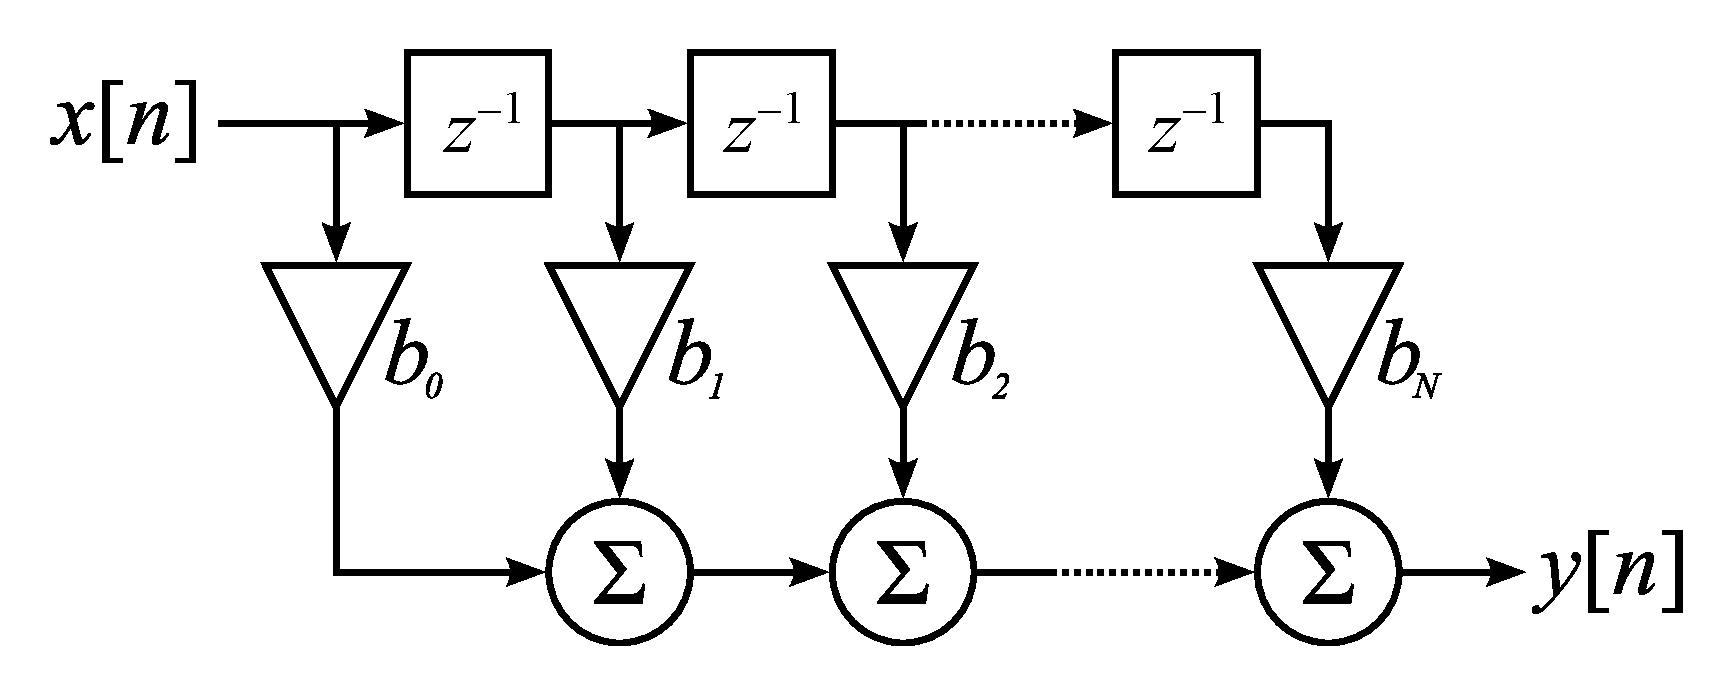
\includegraphics[width=300pt]{figures/chap3-fir-filter.pdf}
    \caption[Estrutura genérica de um filtro FIR]{Estrutura genérica de um filtro FIR. Extraída de \cite{Blanchard2008}.}
    \label{fig:firfilter}
\end{figure}

O segundo tipo de filtro diz respeito àqueles cuja resposta depende não apenas dos valores da entrada mas também dos valores da própria saída. Em outras palavras, há um laço de \emph{feedback} que conecta a saída a uma parte da entrada do filtro, realimentando-o. Isto implica dizer que sua resposta ao impulso será potencialmente infinita. Por esse motivo aliás, o filtro pode ser instável no sentido BIBO (\emph{bounded input, bounded output}), isto é, pode ter saída de valor ilimitado para uma entrada de valor limitado. A figura \ref{fig:iirfilter} mostra a estrutura genérica de um filtro IIR.

\begin{figure}[ht!]
    \centering
    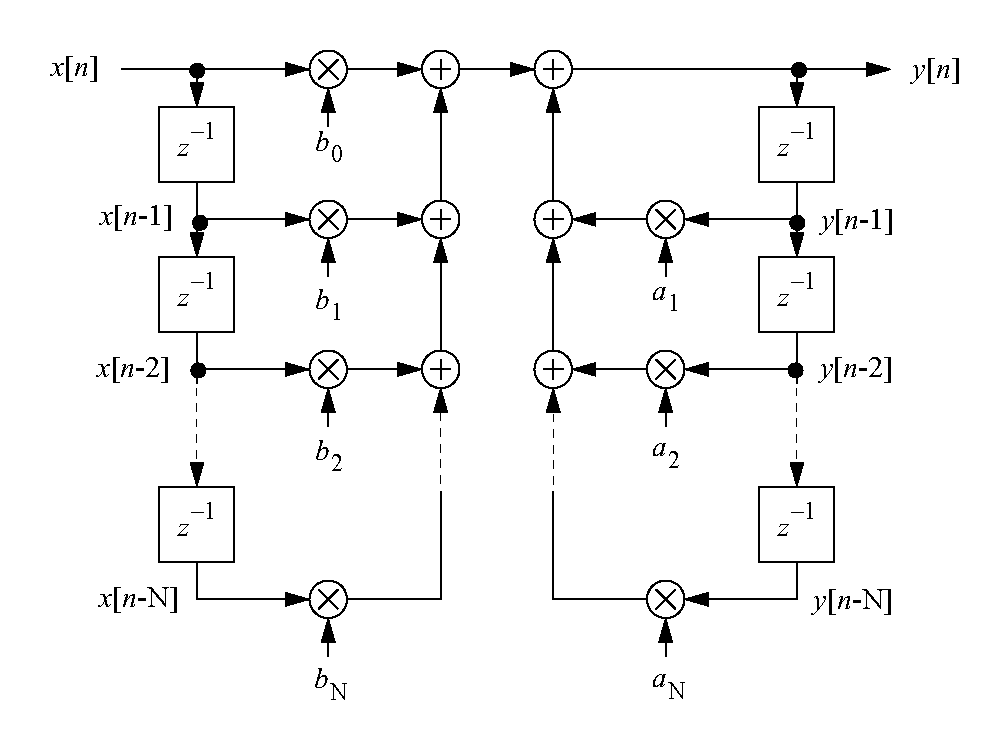
\includegraphics[width=400pt]{figures/chap3-iir-filter.pdf}
    \caption[Estrutura genérica de um filtro IIR]{Estrutura genérica de um filtro IIR.}
    \label{fig:iirfilter}
\end{figure}

Não se pretende aqui discutir em detalhe os critérios de estabilidade e causalidade de um filtro, questões estas que estão diretamente relacionadas com a região de convergência escolhida para a transformada z do sistema. Entretanto, vale mencionar que um filtro será realizável se ele for causal (saída zero para tempos menores que zero) e estável (saída limitada para entrada limitada). Todos os filtros projetados neste trabalho são realizáveis, de modo que podemos nos concentrar no projeto em si e não abordar estes princípios explicitamente.

Filtros FIR podem ser projetados de várias maneiras, sendo algumas delas: truncagem da resposta ideal, alocação de zeros no plano z e amostragem em frequência. Num primeiro momento, apresentaremos uma metodologia especial desenvolvida por Lynn (\cite{Lynn1971}, \cite{Lynn1977}), em que são projetados filtros com coeficientes inteiros. Consecutivamente, será vista a técnica de truncagem da resposta ideal por janelas. Esta última é necessária para o algoritmo de reamostragem que será visto no capítulo \ref{chap:chapter6}. Ao final da seção, será abordada questão de projeto de filtros IIR, necessária para o condicionamento do sinal de ECG (remoção de ruido/interferência).

\subsection*{Projeto de filtros FIR com coeficientes inteiros}
Lynn \cite{Lynn1977} propõe uma técnica de projeto de filtros FIR que proporciona vantagens sobre outras técnicas em termos de eficiência computacional, embora seja um tanto restritiva em termos de qualidade da resposta desejada. A principal vantagem desses filtros é que sua equação de diferenças possui apenas coeficientes inteiros, de modo que a filtragem possa ser realizada por multiplicações e adições inteiras, em vez de por operação em ponto-flutuante. Dependendo do caso, pode-se até realizar as operações de multiplicação por meio de deslocamentos de bits, tornando a filtragem ainda mais rápida.

A função de transferência base para um filtro passa-baixas nesta técnica é da seguinte forma:
\begin{equation}
     H_{lp}(z) = \frac{1-z^{-m}}{1-z^{-1}}.
     \label{equ:intlp}
\end{equation}
O termo denominador indica que há um pólo em $z=1$ (ou frequência $\omega =0$ rad), enquanto o termo numerador indica que existem $m$ zeros uniformemente distribuídos ao longo do círculo unitário, com ângulo de separação igual a $(2\pi/m)$ radianos. O zero em $z=1$ cancela o pólo no mesmo local, de modo que o filtro possui comportamento FIR. Não obstante, o pólo em $z=1$ introduz um termo em $y[n-1]$ na equação de diferenças, o que é claramente uma característica de filtros IIR. Esta também é uma vantagem, pois normalmente a equação de diferenças da versão IIR de um filtro FIR, quando ela existe, possui menos termos e, por consequência, necessita de menos operações (isto faz sentido porque o laço de realimentação reduz a dependência explícita da saída em termos da entrada).

A primeira coluna da figura \ref{fig:zeros} ilustra a disposição de zeros da equação \ref{equ:intlp} no plano z para alguns valores de $m$. Como o zero em $z=1$ é cancelado pelo pólo coincidente, a resposta em frequência do filtro tem seu pico neste ponto, em vez de cair a zero. A figura \ref{fig:freqzlp} mostra o módulo de $H_{lp}(z)$ quando $m=3$. A escala de frequências está normalizada no intervalo 0 a 1, correspondendo a 0 e $\pi$ radianos. Nota-se que a frequência onde o módulo cai a zero é igual a $(2\pi/3)$, ou, na escala da figura, $0,\overline{6}$. Nota-se também que o ganho do filtro na banda passante é o próprio valor de $m$, neste caso igual a 3. Isto vale para qualquer filtro no formato da Eq. \ref{equ:intlp}.

\begin{figure}[ht!]
    \centering
    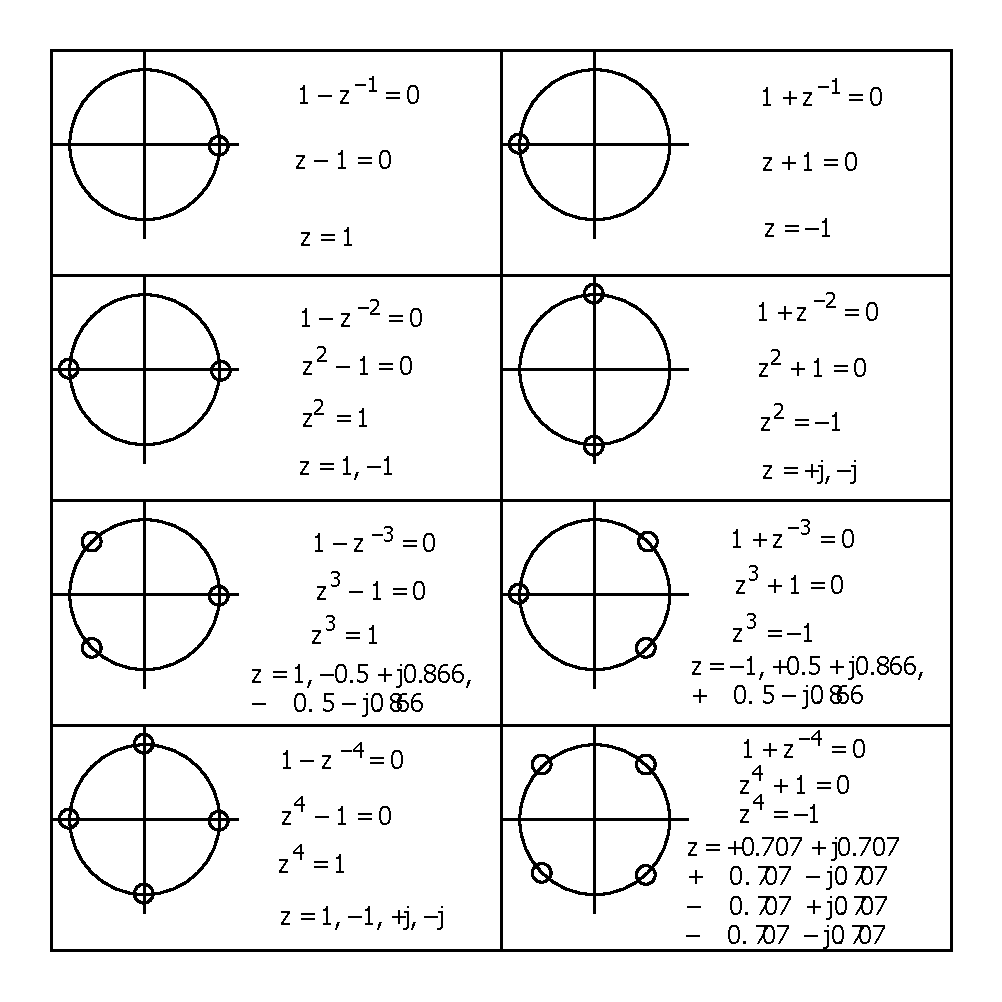
\includegraphics[width=400pt]{figures/chap3-zeros.pdf}
    \caption[Raízes de $1-z^{-m}$ e de $1+z^{-m}$]{Raízes de $1-z^{-m}$ (primeira coluna) e de $1+z^{-m}$ (segunda coluna). Extraída de \cite{Tompkins1993}}
    \label{fig:zeros}
\end{figure}

\begin{figure}[ht!]
    \centering
    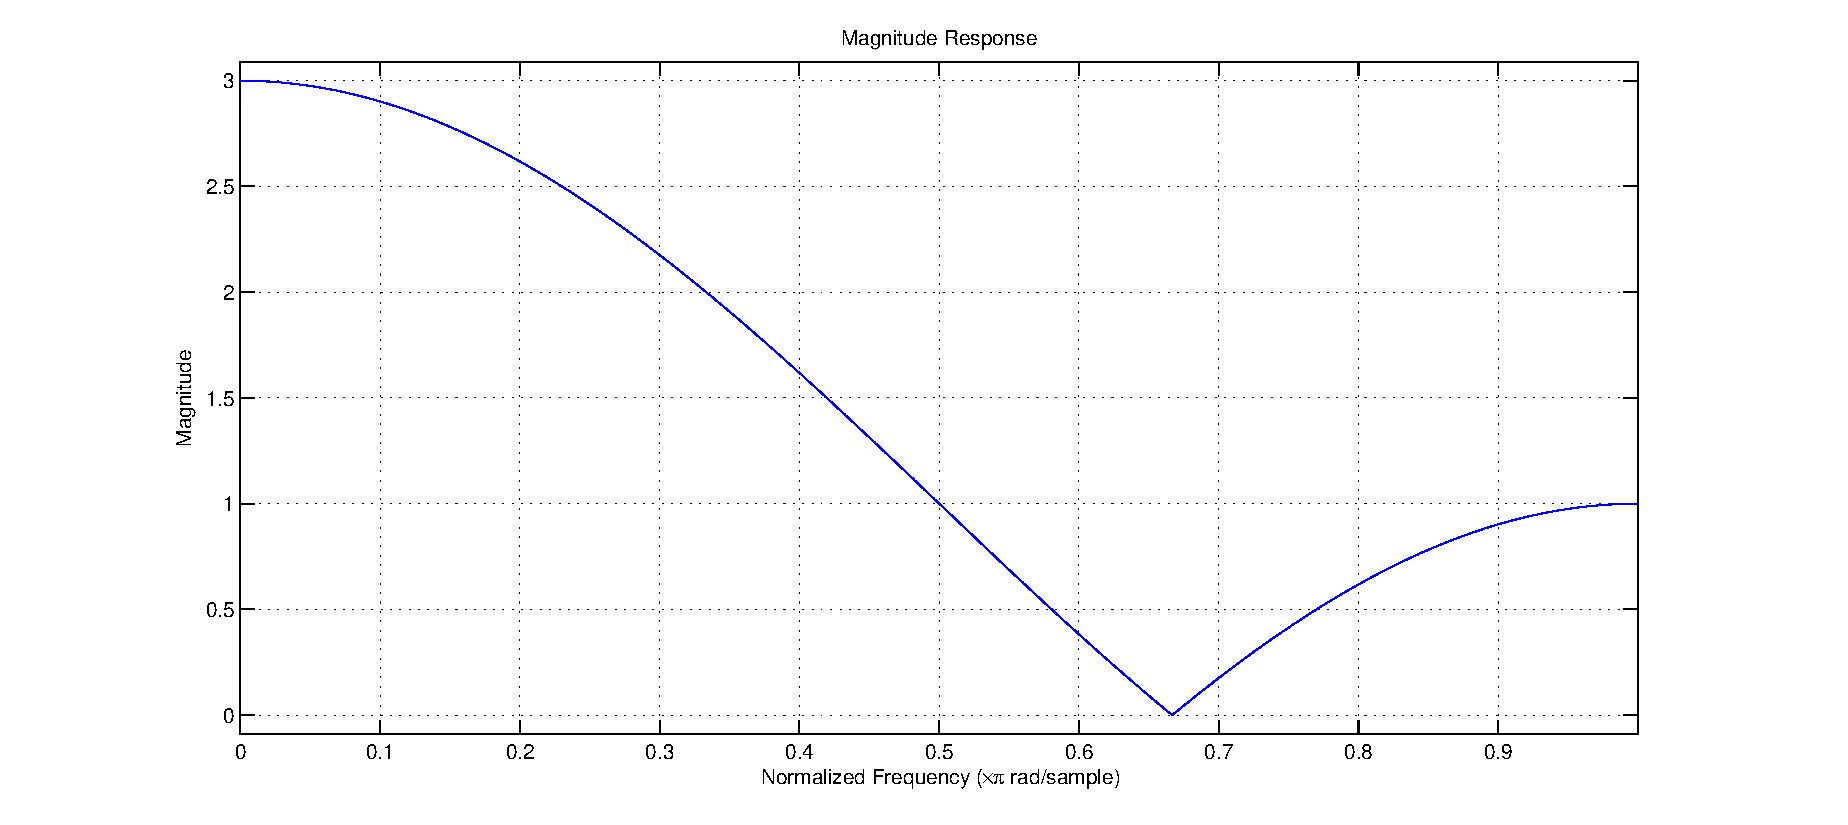
\includegraphics[width=500pt]{figures/chap3-freqz-lp.pdf}
    \caption[Resposta em frequência do filtro passa-baixas para $m=3$]{Resposta em frequência do filtro passa-baixas para $m=3$. Produzida no MATLAB}
    \label{fig:freqzlp}
\end{figure}

A função de transferência do passa-altas é similar, mas apresenta duas formas:
\begin{equation}
     H_{hp_1}(z) = \frac{1-z^{-m}}{1+z^{-1}}, \quad \quad
     H_{hp_2}(z) = \frac{1+z^{-m}}{1+z^{-1}}.
     \label{equ:inthp}
\end{equation}
Aqui o denominador indica que o pólo está em $z=-1$ (ou frequência $\omega =\pi$ rad). Na segunda forma, o numerador implica uma rotação na disposição de zeros no círculo unitário, em relação à primeira forma, conforme ilustra a segunda coluna da figura \ref{fig:zeros}. Isto significa que, para $m$ par, deve-se usar $H_{hp_1}(z)$ no projeto do passa-altas e usar $H_{hp_2}(z)$ somente quando $m$ for ímpar. A figura \ref{fig:freqzhp} mostra o módulo de $H_{hp_2}(z)$ quando $m=3$.

\begin{figure}[ht!]
    \centering
    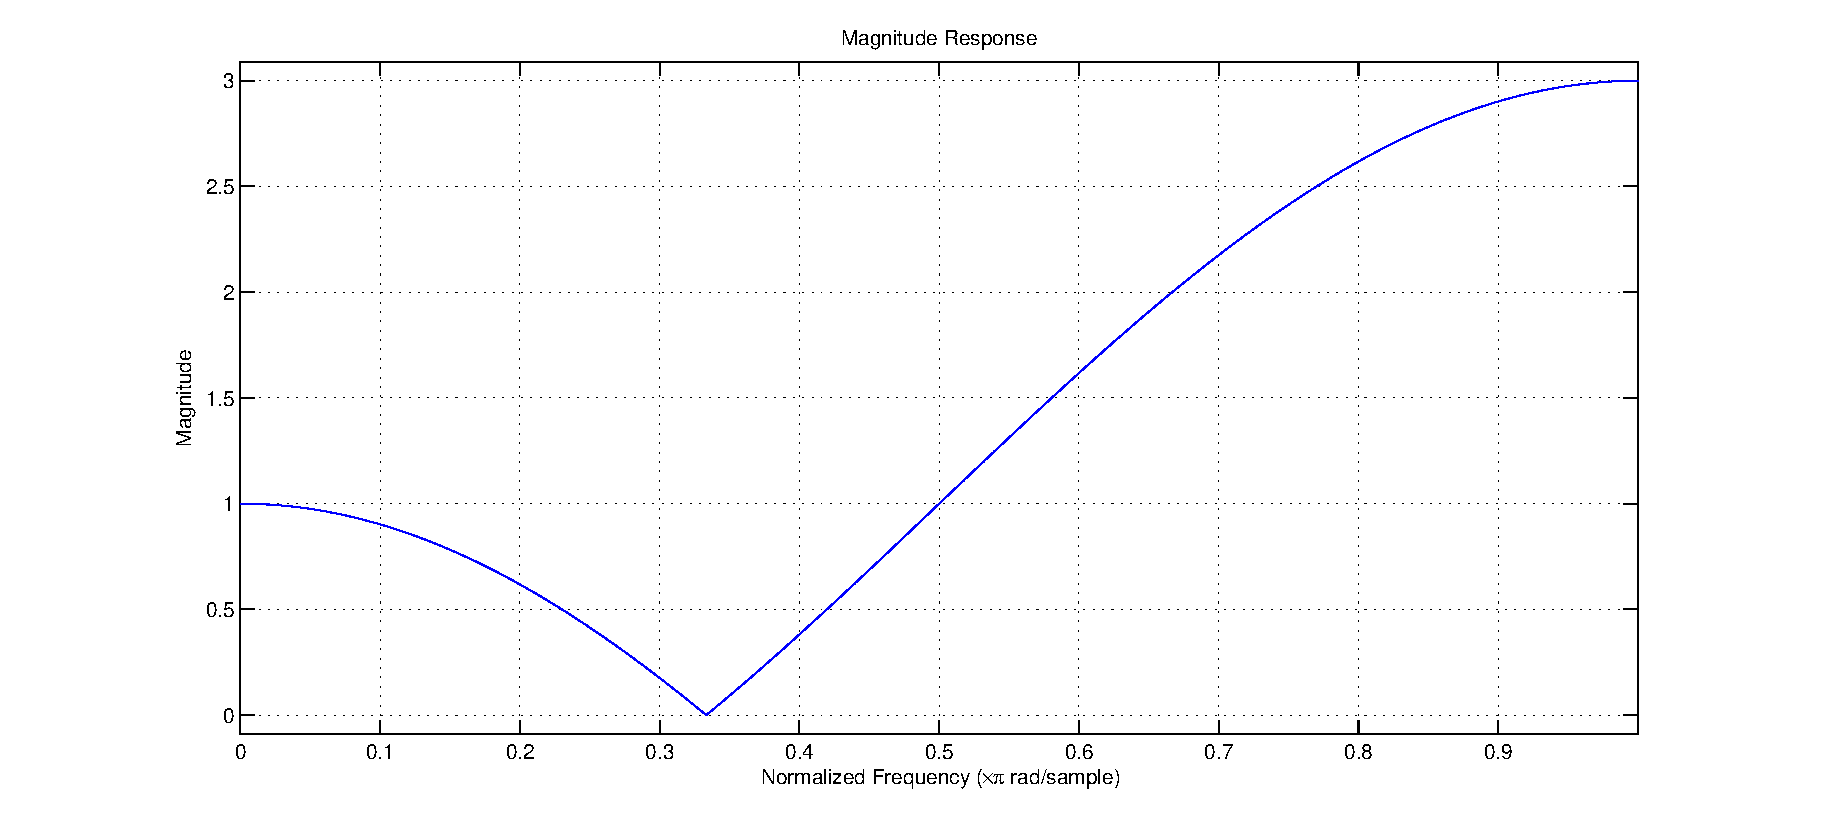
\includegraphics[width=500pt]{figures/chap3-freqz-hp.pdf}
    \caption[Resposta em frequência do filtro passa-altas para $m=3$]{Resposta em frequência do filtro passa-altas para $m=3$. Produzida no MATLAB}
    \label{fig:freqzhp}
\end{figure}

O parâmetro $m$ deve ser cuidadosamente escolhido para atender a uma determinada especificação. Nesta técnica de projeto, não há como satisfazer uma especificação arbitrária, pois a localização de pólos e zeros no círculo unitário é bastante restritiva. Contudo, dadas uma frequência de corte $\omega_c$ e a magnitude de $H(e^{j\omega})$ nesta frequência, é possível encontrar um valor de $m$ que atenda a essas restrições, mesmo que outras características da resposta em frequência permaneçam irrestritas. Assim sendo, deve-se resolver a equação
\begin{equation}
     \left.|H(e^{j\omega})|\right|_{\omega=\omega_c} = mC,
     \label{equ:solvem}
\end{equation}
onde $C$ é a magnitude desejada (com respeito a um ganho unitário) em $\omega_c$ e $m$ constitui o ganho do filtro na banda passante. De maneira similar, foi realizada a análise da função de transferência de ordem $N$, que nada mais é do que a composição de $N$ filtros iguais em cascata:
\begin{equation}
     H^N_{lp}(z) = \left(\frac{1-z^{-m}}{1-z^{-1}}\right)^N
\end{equation}
e
\begin{equation}
     H^N_{hp_1}(z) = \left(\frac{1-z^{-m}}{1+z^{-1}}\right)^N, \quad
     H^N_{hp_2}(z) = \left(\frac{1+z^{-m}}{1+z^{-1}}\right)^N.
\end{equation}

A equação \ref{equ:solvem} pode ser expressa como uma equação trigonométrica, usando a função seno, mas não possui solução analítica simples. Portanto, neste trabalho utilizou-se o resolvedor numérico do MATLAB (função \texttt{vpasolve}) e encontrou-se valores de $\omega_c$ para diversas combinações de $m$ e $C$. Variou-se $m$ no intervalo $[2,200]$ e $C$ possuía um de três valores, correspondendo às atenuações de -3dB, -6dB e -24dB, relativas ao ganho $m$ do filtro. A equação trigonométrica fornecida ao resolvedor vem da substituição $z=e^{j\omega}$ em $H^N_{lp}(z)$ e é dada por
\begin{equation}
     \left|\frac{\sin \left(m\frac{\omega}{2}\right)} {m\sin\left(\frac{\omega}{2}\right)}\right|^N = C.
\end{equation}
Com os valores de $m$ e $\omega_c$, para cada atenuação desejada e ordem $N$ do filtro, construiu-se um modelo de regressão que nos dá $m$ em função de $\omega_c$ e estimou-se os parâmetros do modelo usando a função \texttt{fitnlm} do MATLAB. Por fim, foi encontrado um modelo de regressão que expressa $m$ em função de $\omega_c$ e $N$, para $1\leq N \leq 10$. Abaixo estão as expressões encontrdas:
\begin{equation}
     m = \left\{
     \begin{array}{l l}
         \frac{0.91823\pi}{\omega_c\sqrt{N+0.072177}} & \quad \text{aten. de -3dB}\\
         \frac{1.2992\pi}{\omega_c\sqrt{N+0.15023}} & \quad \text{aten. de -6dB}\\
         \frac{1.732\pi}{\omega_c\sqrt{N+0.28356}} & \quad \text{aten. de -24dB}\\
         \frac{2\pi}{\omega_c} & \quad \text{aten. de $-\infty$}
     \end{array} \right..
\end{equation}

É importante ressaltar que o mesmo modelo pode ser usado tanto no projeto do passa-baixas quanto no do passa-altas, pois o que muda é a rotação da disposição de zeros no plano z e não o número de zeros que dividem o círculo unitário. (Podemos pensar no passa-altas como um deslocamento de $\pi$ radianos da resposta em frequência do passa-baixas.)

\subsection*{Projeto de filtros FIR por truncagem da resposta ideal}
A segunda maneira de projetar filtros FIR usada neste trabalho advém da construção da resposta impulsiva do filtro com base numa resposta ideal. A resposta em frequência de um filtro passa-baixas ideal é dada por:
\begin{equation}
     H_d(e^{j\omega}) = \left\{
     \begin{array}{l l}
         e^{j\omega\alpha} & \quad |\omega| \leq \omega_c\\
         0                 & \quad \omega_c \leq |\omega| \leq \pi
     \end{array} \right.,
\end{equation}
periódica com período $2\pi$. O parâmetro $\alpha$ é um fator de fase e garante, no domínio tempo, o atraso necessário para tornar o filtro causal. A figura \ref{fig:ideal} mostra um esboço da magnitude de $H_d(e^{j\omega})$. A resposta impulsiva do filtro é dada pela aplicação da transformada inversa de Fourier de tempo discreto:
\begin{equation}
     h_d[n] = \frac{1}{2\pi}\int_{-\omega_c}^{\omega_c} e^{j\omega\alpha}e^{j\omega n} = \frac{\sin \left( \omega_c \left(n-\alpha\right) \right)}{\pi \left(n-\alpha\right)}.
     \label{equ:impresp}
\end{equation}

\begin{figure}[ht!]
    \centering
    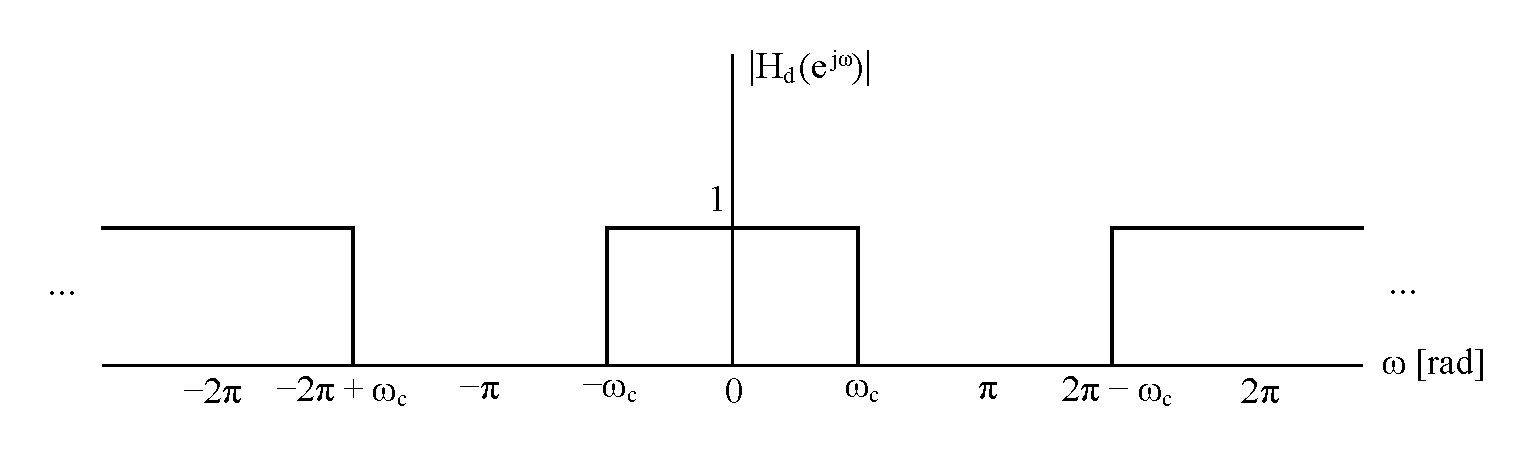
\includegraphics[width=400pt]{figures/chap3-ideal-lowpass.pdf}
    \caption[Resposta em frequência do filtro passa-baixas ideal]{Resposta em frequência do filtro passa-baixas ideal.}
    \label{fig:ideal}
\end{figure}

Desejamos truncar $h_d[n]$ num intervalo de tamanho $M$, com $\alpha=\frac{M}{2}$. Para tanto, utilizamos uma ``janela'' delimitadora, $w[n]$. Assim, tem-se
\begin{equation}
     h[n] = h_d[n]w[n], \quad 0\leq n \leq M,
     \label{equ:trunc}
\end{equation}
que no domínio frequência equivale a uma convolução de $H_d(e^{j\omega})$ com $W(e^{j\omega})$, e implica num ``espalhamento'' de energia da resposta ideal. A figura \ref{fig:design} mostra um esboço da magnitude de $H(e^{j\omega})$ juntamente com a resposta ideal (em traço segmentado). A figura também revela os diversos parâmetros utilizados no projeto do filtro.

\begin{figure}[ht!]
    \centering
    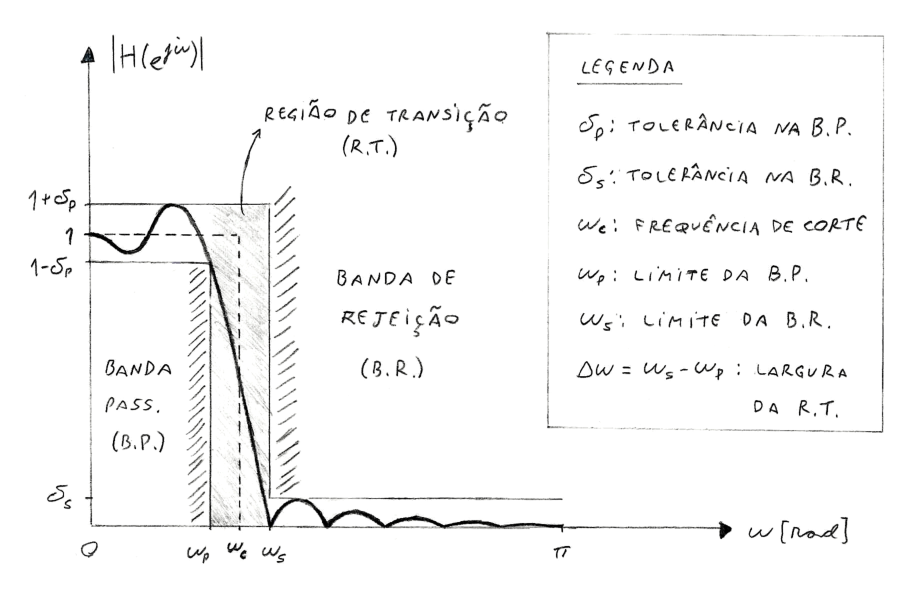
\includegraphics[width=350pt]{figures/chap3-design-lowpass.pdf}
    \caption[Especificações de projeto do filtro passa-baixas realizável]{Especificações de projeto do filtro passa-baixas realizável.}
    \label{fig:design}
\end{figure}

Visando reduzir o espalhamento de energia o tanto quanto possível, diversos tipos de janela foram propostos na literatura de processamento de sinais (\cite{Harris1978}, \cite{Kaiser1980}), cada uma com suas características. As características mais importantes de uma janela, do ponto de vista de sua resposta em frequência, são a largura do lóbulo principal e a atenuação média da banda de rejeição. Alguns tipos comuns de janela utilizados são: retangular, Bartlett (ou triangular), Hanning, Hamming, Blackman e Kaiser.

Os passos para se obter a resposta desejada de um filtro passa-baixas digital são:
\begin{enumerate}
    \item Tomar a menor tolerância entre as das bandas passante e de rejeição: $\delta = min(\delta_p,\delta_s)$;
    \item Calcular a atenuação requerida em decibéis, com base na tolerância: $A = -20\log_{10}(\delta)$;
    \item Escolher um tipo de janela que satisfaça a atenuação desejada; 
    \item Calcular a largura da região de transição: $\Delta\omega = |\omega_s-\omega_p|$;
    \item Descobrir o tamanho da resposta com base em $\Delta\omega$ e na janela: $M = f_w(\Delta\omega)$; e\footnote{a função $f_w$ é apenas uma maneira de dizer que existe uma relação entre $\Delta\omega$ e $M$}
    \item Calcular $h[n]$ usando as Eqs. \ref{equ:impresp} e \ref{equ:trunc}.
\end{enumerate}


\subsection*{Conversão de filtros IIR analógicos}
Historicamente, o projeto de filtros IIR digitais sempre teve como base as técnicas de projeto desenvolvidas no mundo contínuo, pois estas já são bastante avançadas e sofisticadas, de modo que é vantajoso reaproveitá-las no mundo discreto em vez de criar um novo ferramental ``a partir do zero''. A conversão da resposta impulsiva ou em frequência de um filtro de tempo contínuo para a resposta de um filtro de tempo discreto pode ser alcançada através de um dos seguintes procedimentos: invariância ao impulso (do inglês, \emph{impulse invariance}) ou transformação bilinear.

Abaixo está um condensado da segunda técnica supracitada, já que é a mais comumente utilizada em ferramentas computacionais de projeto de filtros, como o MATLAB. Na verdade, o que segue é apenas uma elucidação do procedimento de projeto. Diferentemente do caso FIR, em que se havia uma fórmula simples para obtenção da resposta do filtro, o projeto dos filtros IIR empregados neste trabalho será realizado com auxílio do MATLAB, conforme será visto no capítulo \ref{chap:chapter6}.

A transformação bilinear é dada pela substituição
\begin{equation}
     s = \frac{2}{T_d} \left(\frac{1-z^{-1}}{1+z^{-1}}\right),
     \label{equ:bilin}
\end{equation}
onde $T_d$ é um parâmetro associado à passagem do tempo contínuo para tempo discreto. Essa transformação mapeia o eixo $j\Omega$ do plano $s$ no círculo unitário do plano $z$. Isto é, mapeia $\Omega$ no intervalo $(-\infty,+\infty)$ para $\omega$ no intervalo $[-\pi,+\pi]$, sendo portanto não-linear. Por este fato, ela provoca uma distorção das frequências, conforme evidencia a relação
\begin{equation}
     \omega = \frac{2}{T_d} \arctan\left(\Omega \frac{T_d}{2}\right).
     \label{equ:warp}
\end{equation}

No projeto de um filtro IIR, é necessário converter as frequências especificadas ($\omega_p$ e $\omega_s$) no mundo digital para o seu correspondente contínuo, usando a Eq. \ref{equ:warp}. As tolerâncias ($\delta_p$ e $\delta_s$) não sofrem alteração. Com as especificações no mundo contínuo, determina-se a função de transferência do filtro analógico, que pode ser do tipo Butterworth, Chebyshev I, Chebyshev II ou elíptico, e finalmente faz-se a conversão da resposta para o mundo discreto usando a Eq. \ref{equ:bilin}.


\section{Resumo}
Este capítulo, que pode à primeira vista parecer extenso, assenta as peças necessárias ao entendimento dos assuntos vindouros. Aqui foram introduzidos os conceitos de norma, base e produto interno, no contexto de espaços vetoriais. Conceitos estes que dão lugar à questão da aproximação de sinais discretos. Uma interpretação foi apresentada no espaço Euclideano com auxílio da operação de projeção. Logo em seguida, viu-se que a sequência de polinômios de Hermite, assim como o conjunto de funções a ela associado, forma uma base ortonormal para o espaço de funções integráveis ao quadrado. No caso discreto, foi abordada uma técnica especial de cálculo das funções de Hermite que permite aproximação de um sinal discreto por meio de um simples produto matricial.

Depois, algumas transformadas de tempo discreto foram vistas, notadamente a transformada de Fourier de tempo discreto (DTFT) e a transformada z. Viu-se como é possível representar a equação de diferenças de um sitema linear e invariante no tempo (LIT) por meio da transformada z e que esta representação permite fácil identificação dos pólos e zeros do sistema. Ainda, o plano z oferece uma ferramenta imprescindível de análise de estabilidade e causalidade desses sistemas, bem como facilita o projeto de filtros, conforme visto na seção subsequente.

Existem diversas maneiras de se projetar filtros FIR, duas das quais foram discutidas na seção \ref{sec:filterdesign}. A primeira, tocante ao projeto de filtros com coeficientes inteiros, forneceu um algoritmo para determinação da função de transferência de filtros passa-baixa e passa-alta com coeficientes inteiros. Depois, foi visto o projeto de um filtro passa-baixa com base na truncagem de sua resposta ideal no domínio tempo. Essa truncagem se dá pelo uso de janelas delimitadoras e resulta em um algoritmo para o cálculo da resposta impulsiva do filtro. Ainda nesta seção teve lugar um breve discurso sobre a conversão de filtros IIR analógicos para o caso discreto, com ênfase na transformação bilinear.